\section{Transport-layer protocols}

\begin{knBox}
    {Transport layer address}
    An application is identified by \texttt{(IP address, port number)}.
\end{knBox}

\subsection{User Datagram Protocol (UDP)}

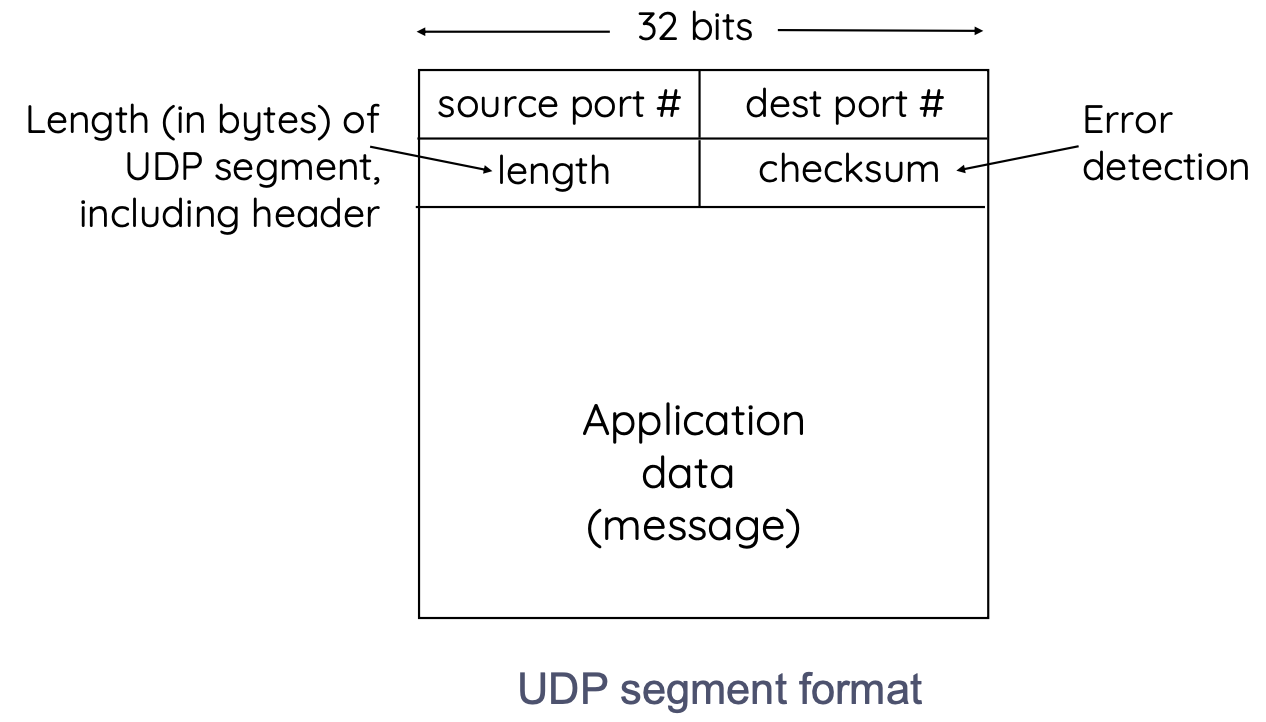
\includegraphics[width=0.5\textwidth]{images/m04-l01-1.png}

\begin{theorem}
    {Checksums (Transport layer)}
    Detect errors in transmitted segments.

    \begin{itemize}
        \item Sender: compute checksum, put in UDP segment
        \item Receiver: compute checksum, check against received checksum
    \end{itemize}

    \textbf{Computation:}

    \begin{itemize}
        \item For each word, add them together, wrap around any overflow (add overflow back)
        \item Take 1's complement of the sum (flip bits)
        \item If checksum + sum = all 1's $\implies$ no error detected
    \end{itemize}

    \textbf{Error detection:}
    \begin{itemize}
        \item $\checkmark$ One / odd number of bits flipped
        \item $\checkmark$ Two bits in different columns flipped
        \item $\checkmark$ Two bits in same columns flipped same direction
        \item $\times$ Two bits of same columns flipped different direction
    \end{itemize}
\end{theorem}

\begin{definition}
    {Principles of Reliable Data Transfer}

    The main two principles are to have reliable:
    \begin{itemize}
        \item \textbf{Abstraction:} Reliable data transfer over an unreliable channel
        \item \textbf{Implementation:} Use acknowledgements and timeouts
    \end{itemize}

    Things that could go wrong includes \textit{corrputed, lost, reordered and duplicated} segments.
\end{definition}

ACK is short for \textbf{acknowledgement}.

NAK is short for \textbf{negative acknowledgement}.

\subsection{Reliable Data Transfer}

\begin{theorem}
    {Alternating Bit Protocol (ABP)}

    Attributes: \textit{Timeout}

    \begin{itemize}
        \item Stop-and-wait protocol
        \item Sequence numbers: 0, 1
        \item Sender waits for ACK/NAK before sending next segment
        \item If timeout, resend segment
    \end{itemize}
\end{theorem}

\sectionbar{M04-L04}

\subsubsection{Sliding window protocols}

\begin{knBox}
    {Cumulative ACKs}
    An ACK for sequence number $k$ acknowledges receipt of \textbf{all prior segments}.
\end{knBox}

\begin{theorem}
    {Go-Back-N (GBN) Protocol}

    Attributes: \textit{Timeout, Window size $N$, sequence number bits $k$}

    \begin{itemize}
        \item Sender can send $N$ segments at once
        \item Sender receiving an ACK will slide it's window forward to the next unACKed segment
        \item Receiver has a \textbf{single}, in-order expected sequence number and sends cumulative ACKs
        \item If sender receives NAK or timeout, it resends all segments in the current sliding window
        \item The maximum window size is $N \leq 2^k - 1$ to avoid sequence number overlap
    \end{itemize}

    Visualization \href{https://media.pearsoncmg.com/aw/ecs_kurose_compnetwork_7/cw/content/interactiveanimations/go-back-n-protocol/index.html}{here}
\end{theorem}

\sectionbar{M04-L05}

\begin{theorem}
    {Selective Repeat (SR) Protocol}

    Attributes: \textit{Timeout, Window size $N$, sequence number bits $k$}

    \begin{itemize}
        \item Sender can send $N$ segments at once
        \item Sender receiving an ACK will slide it's window forward to the next unACKed segment
        \item Receiver accepts out-of-order segments, buffers them, and sends individual ACKs
        \item If sender receives NAK or timeout, it resends only the specific segment
        \item The maximum window size is $N \leq 2^{k-1}$ to avoid sequence number overlap
    \end{itemize}

    Visualization \href{https://media.pearsoncmg.com/aw/ecs_kurose_compnetwork_7/cw/content/interactiveanimations/selective-repeat-protocol/index.html}{here}
\end{theorem}